% !TEX encoding = UTF-8 Unicode
% -*- coding: UTF-8; -*-
% vim: set fenc=utf-8

\section{Komponenta editoru}\label{sec:komponentaEditoru}

Komponenta editoru je hlavním částí aplikace, umožňuje uživatelům společně upravovat dokumenty ve skutečném čase díky použití algoritmu \gls{OT} (více o volbě algoritmu v sekci~\ref{sec:synchronizaceEditovanéhoTextu}).
Komponenta tento algoritmus implementuje a poskytuje rozhraní pro jeho použití bez omezení na použité technologii komunikace, či samotné knihovny textového editoru.

Komponentu editoru rozdělíme na dvě části, část klientská a část serverová.

\subsection{Klientská část komponenty}\label{subsec:klientskáČást}

Klientská část musí komunikovat se zvoleným textovým editorem, zachytávat uživatelův vstup a následně ho převést na abstraktní object operace, který lze dále použít v rámci algoritmu \gls{OT}.
Tato část také musí umět komunikovat pomocí zvolené komunikační technologii s částí serverovou (propagace jednotlivých Operací mezi uživateli).

Jádrem této části je třída \texttt{EditorClient}, která dědí od třídy \texttt{Client} z knihovny OT.js.
Dědí vlastnosti a metody implementující jádro algoritmu \gls{OT}, jako je například udržování čísla revize a transformace přijatých operací v případě existence nepotvrzené vlastní operace.
Třída \texttt{Client} a tedy i třída \texttt{EditorClient} je navržena podle návrhového vzoru stav a může nabývat 3 stavů (viz stavový diagram na obrázku~\ref{fig:stavovyDiagram}).

\begin{figure}[ht!]
    \centering
    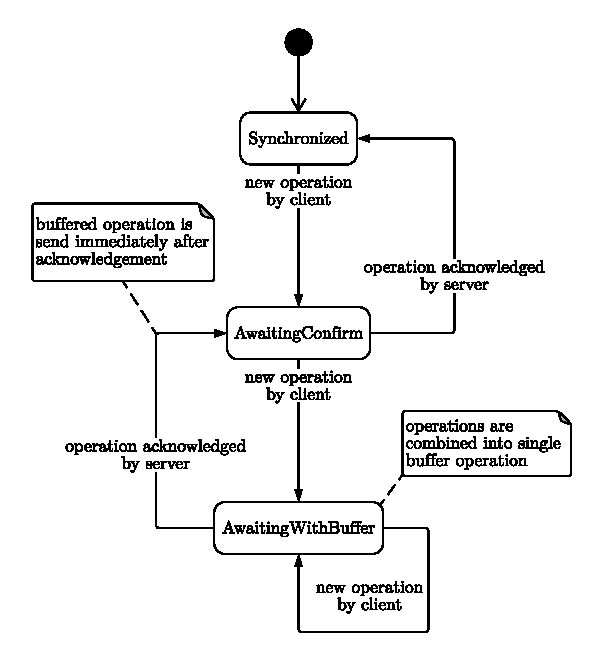
\includegraphics[width=\textwidth]{partials/navrh/stavovyDiagram.pdf}
    \caption{Stavový diagram klientské části komponenty}\label{fig:stavovyDiagram}
\end{figure}

Třída \texttt{EditorClient} očekává implementaci třídy \texttt{AbstractEditorAdapter} (respektive \texttt{AbstractServerAdapter}), která slouží jako rozhraní pro komunikaci s textovým editorem (respektive serverovou částí).
Použití abstraktních tříd umožňuje změnu jednotlivých částí aplikace (změna komunikační technologie, či knihovna textového editoru) a to bez nutnosti zásahu do logiky pro synchronizaci samotných textů.

Tyto abstraktní třídy jsou potomky třídy \texttt{EventEmitter}, která je ustálenou implementací návrhového vzory Pozorovatel (anglicky Observer) pro jazyk Javascript.
Rozhraní \texttt{EventEmitter} umožňuje třídě \texttt{EditorClient} naslouchat jednotlivým událostem, ke kterým dochází v implementacích zmíněných abstraktních tříd (jako je například změna pozice kursoru, či přijatá operace od serveru).
Seznam jednotlivých událostí je možné pozorovat na diagramu~\ref{fig:AbstractEditorAdapter} (respektive~\ref{fig:AbstractServerAdapter}).

\begin{figure}[ht!]
    \centering
    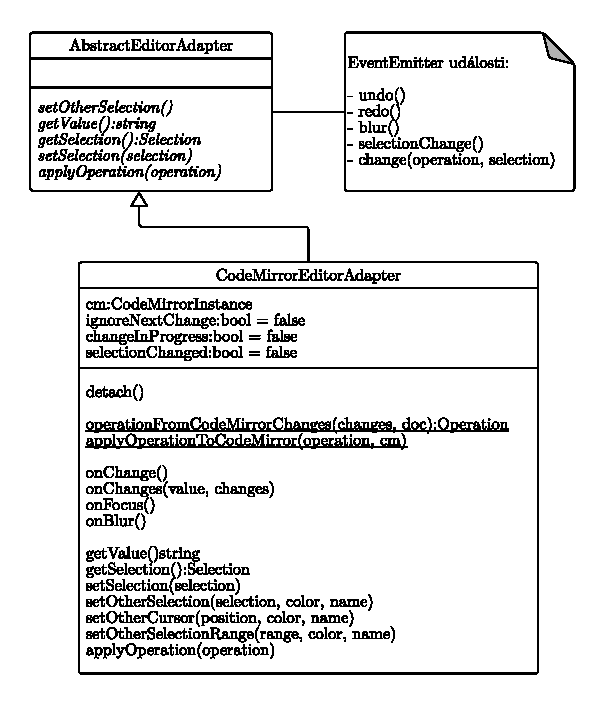
\includegraphics[width=\textwidth]{partials/navrh/AbstractEditorAdapter.pdf}
    \caption{Diagram implementace třídy AbstractEditorAdapter}\label{fig:AbstractEditorAdapter}
\end{figure}

\begin{figure}[ht!]
    \centering
    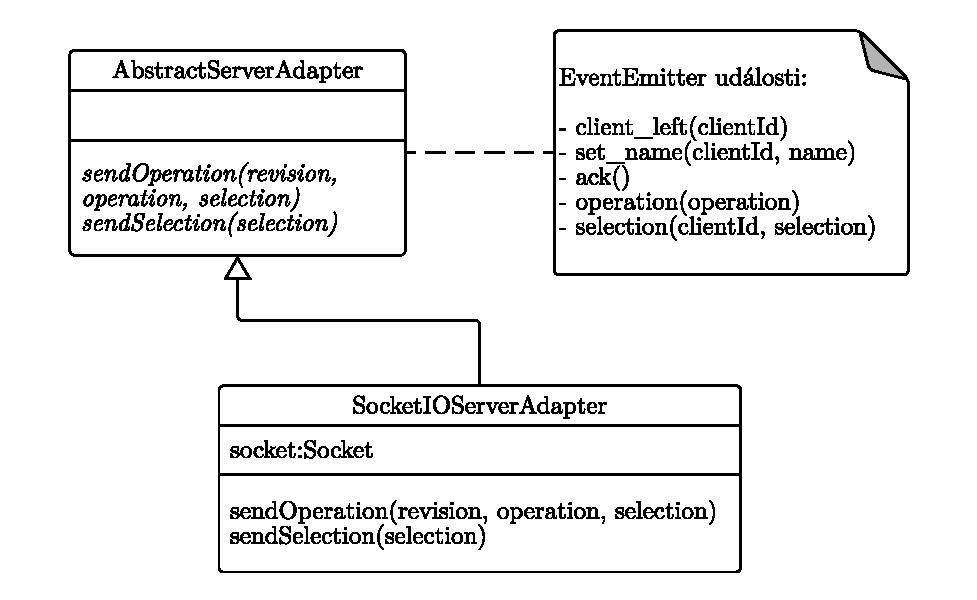
\includegraphics[width=\textwidth]{partials/navrh/AbstractServerAdapter.pdf}
    \caption{Diagram implementace třídy AbstractServerAdapter}\label{fig:AbstractServerAdapter}
\end{figure}

\texttt{EditorClient} také využívá třídu \texttt{UndoManager} z knihovny OT.js, díky kterému lze použít bezpečně funkce zpět a vykonat znovu (pokud jejich odchycení podporuje poskytnutá implementace třídy \texttt{AbstractEditorAdapter}).
Historie je tak zaznamenávána pomocí jednotlivých operací uživatele a nikoly podle změn samotného textu.
Na změnách textu se může podílet více uživatelů najednou a není žádoucí, aby funkce zpět vracela změny provedené jiným než lokálním uživatelem.

\begin{figure}[ht!]
    \centering
    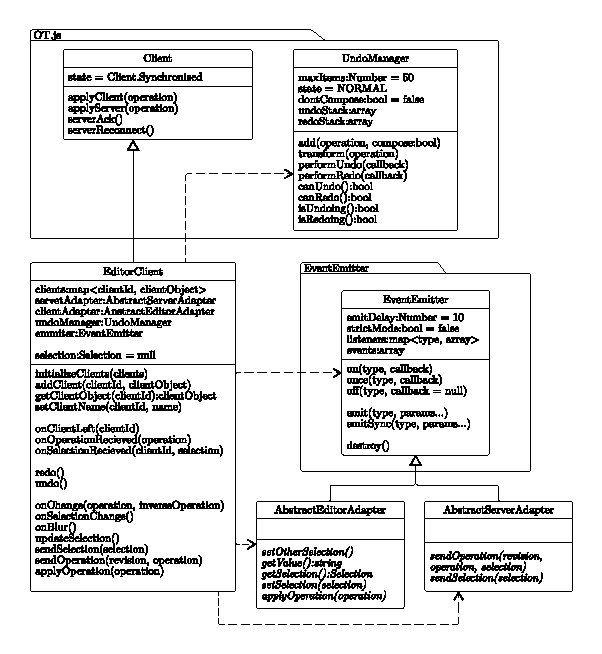
\includegraphics[width=\textwidth]{partials/navrh/EditorClient.pdf}
    \caption{Třídní diagram klientské části komponenty}\label{fig:EditorClient}
\end{figure}

\subsection{Serverová část komponenty}\label{subsec:serverováČást}

Serverová část je odpovědná za propagaci jednotlivých operací mezi klienty připojenými k dokumentu.
Základem této části je třída \texttt{DocumentServer} (reimplementace třídy Server z knihovny OT.js) a v případě navrhovaného prototypu aplikace její potomek \texttt{DocumentSocketIOServer}.

Instance třídy \texttt{DocumentServer} (respektive \texttt{DocumentSocketIOServer}) představuje jeden document a je zodpovědná o implementaci serverové části algoritmu~\gls{OT}.
Musí umět transformovat přijaté revize oproti souběžným, ale již schváleným operacím, a propagovat tuto transformovanou operaci ostatním uživatelům.

Další třídou, kterou je vhodné zmínit je třída \texttt{RoomList}, která udržuje informace o již existujících instancích třídy \texttt{DocumentSocketIOServer}, vytváří nové instance v případě, že pro daný dokument dosud neexistuje, a naslouchá novým socket.io spojení s klienty, které dále předává příslušným instancím třídy \texttt{DocumentServer}.

\begin{figure}[ht!]
    \centering
    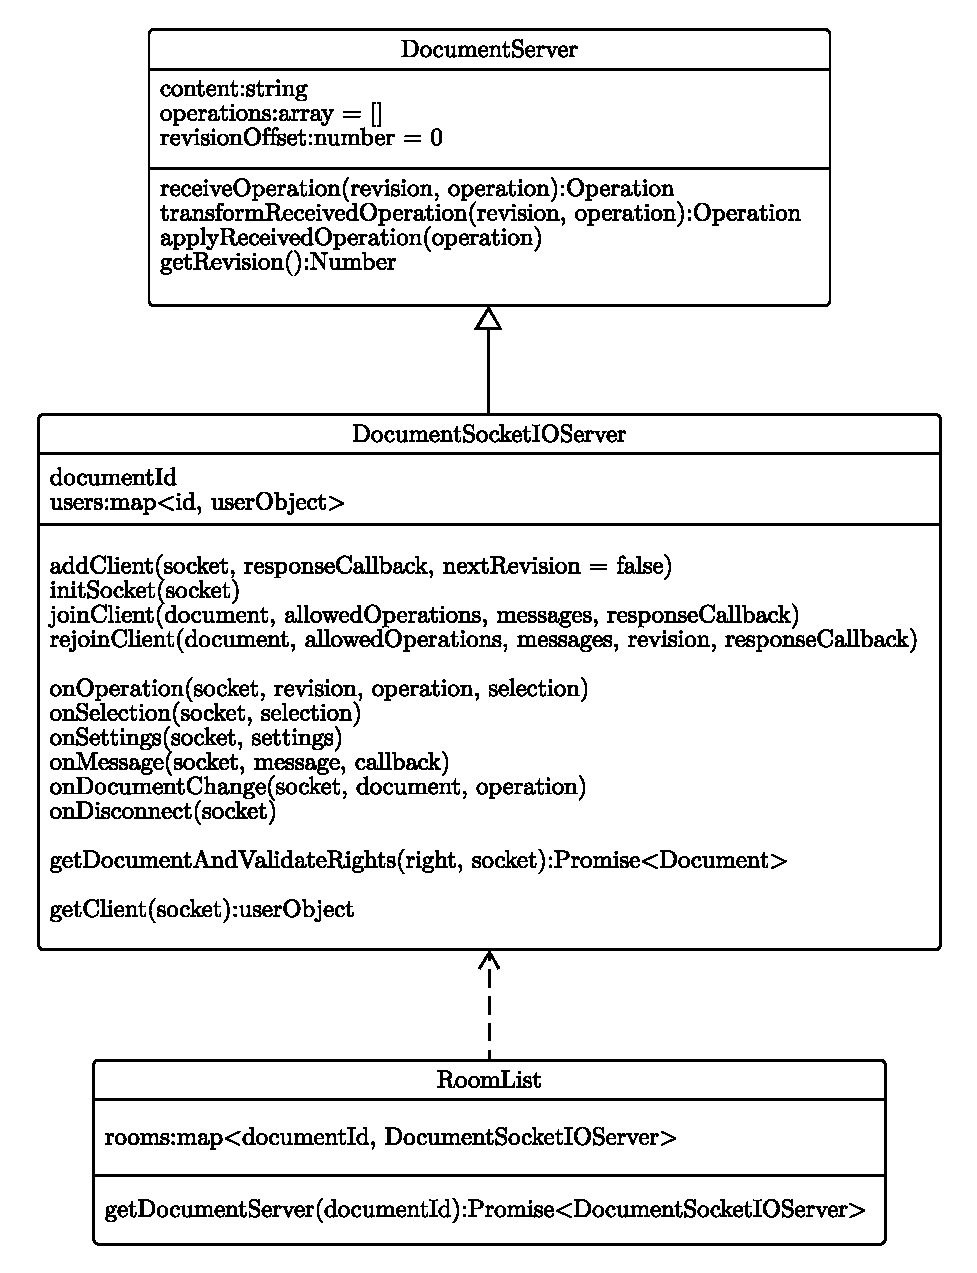
\includegraphics[width=\textwidth]{partials/navrh/DocumentServer.pdf}
    \caption{Třídní diagram serverové části komponenty}\label{fig:DocumentServer}
\end{figure}
